\hsection{The Use of Multivalued Attributes}%
\hsection{Violation:~{T}he Use of Multivalued Attributes}%
\FloatBarrier%
%
\begin{figure}%
\centering%
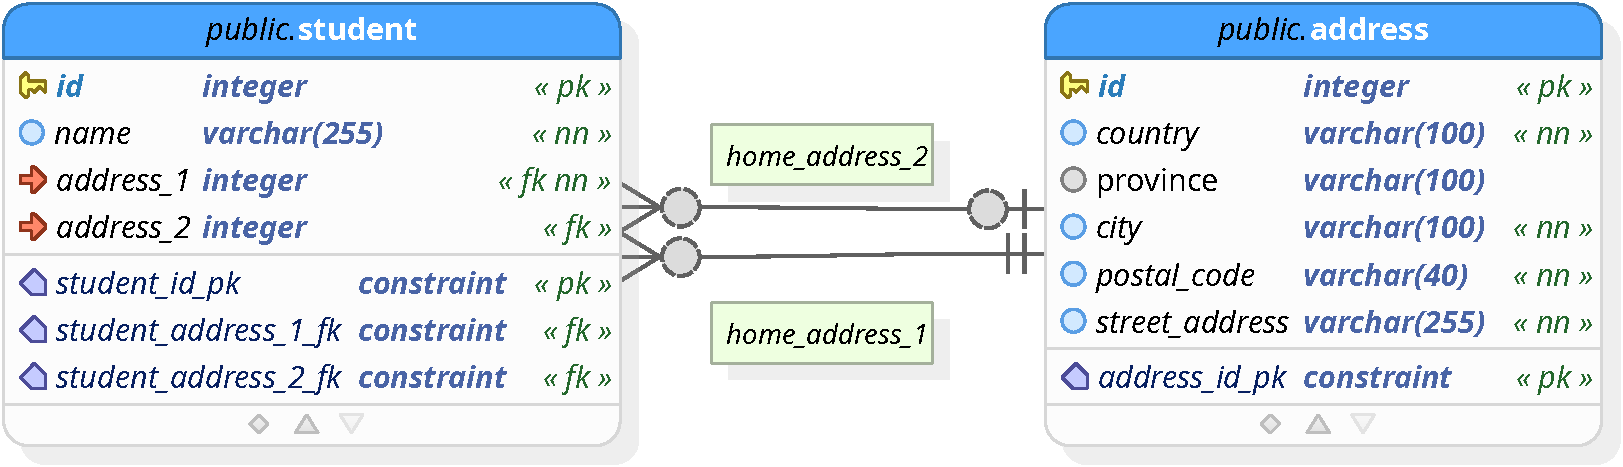
\includegraphics[width=0.85\linewidth]{\currentDir/anomalyMultivalued}%
\caption{A violation of the \pgls{1NF}:~{T}he \sqlil{student} table has two columns with the same semantic, i.e., a repeating group. %
Both columns reference addresses to simulate a multivalued attribute.}%
\label{fig:anomalyMultivalued}%
\end{figure}%
%
\gitExec{}{\databasesCodeRepo}{.}{_scripts_/postgres.sh normalization/1nf/anomaly_multivalued/generated_sql 01_anomalies_database_2001.sql}%
\gitExec{}{\databasesCodeRepo}{.}{_scripts_/postgres.sh normalization/1nf/anomaly_multivalued/generated_sql 03_public_address_table_5071.sql anomalies}%
%
\gitSQL{\databasesCodeRepo}{normalization/1nf/anomaly_multivalued/generated_sql/04_public_student_table_5079.sql}{1nf:anomaly_multivalued:04_public_student_table_5079}{The generated \sql\ code for creating the \sqlil{student} table with two columns for addresses based on \cref{fig:anomalyMultivalued}, which violates the \pgls{1NF}. %
The corresponding \sqlilIdx{REFERENCES} constraints have been omitted here for the sake of brevity.}%
\gitExec{}{\databasesCodeRepo}{.}{_scripts_/postgres.sh normalization/1nf/anomaly_multivalued/generated_sql 04_public_student_table_5079.sql anomalies}%
%
\gitExec{}{\databasesCodeRepo}{.}{_scripts_/postgres.sh normalization/1nf/anomaly_multivalued/generated_sql 05_public_student_student_address_1_fk_constraint_5085.sql anomalies}%
\gitExec{}{\databasesCodeRepo}{.}{_scripts_/postgres.sh normalization/1nf/anomaly_multivalued/generated_sql 06_public_student_student_address_2_fk_constraint_5086.sql anomalies}%
%
\gitSQL{\databasesCodeRepo}{normalization/1nf/anomaly_multivalued/insert.sql}{1nf:anomaly_multivalued:insert}{%
Inserting some data into the tables~\sqlil{student} and~\sqlil{address} in violation of the \pgls{1NF} based on \cref{fig:anomalyMultivalued}.}%
\gitExec{}{\databasesCodeRepo}{.}{_scripts_/postgres.sh normalization/1nf/anomaly_multivalued insert.sql anomalies}%
%
\gitSQLAndOutput{\databasesCodeRepo}{normalization/1nf/anomaly_multivalued}{select.sql}{anomalies}{}{}{postgres.sh}{1nf:anomaly_multivalued:select}{%
Trying to find all the students with at least one address in China, which is harder than necessary, because table \sqlil{student} violates the \pgls{1NF}.}%
%
\gitExec{}{\databasesCodeRepo}{.}{_scripts_/postgres.sh normalization/1nf/anomaly_multivalued cleanup.sql}%
\afterpage{\clearpage}%
%
Let us continue our example from the previous section.
There, we developed a two-table structure for storing addresses of students.
Each student had exactly one address.
But maybe in reality, students can have more than one address.
Let's say their current address, maybe in the university dormitory in a flat rented nearby, and their old home address, i.e., the flat of their parents.
In the model from the previous section, this cannot be implemented.
In \cref{fig:anomalyMultivalued}, the \db\ developer had a very simple idea:
Let's just have two columns for the addresses -- \sqlil{address_1} and \sqlil{address_2} -- in the table~\sqlil{student}.
By doing so, they have violated the \pgls{1NF}.
The table~\sqlil{student} is created based on this model in \cref{lst:1nf:anomaly_multivalued:04_public_student_table_5079}.
We omitted the foreign key \sqlilIdx{REFERENCES} constraints for the sake of brevity.
We also did not print the \sql\ script for creating the table~\sqlil{address}, since it remains the same as in the last section.

The violation of the \pgls{1NF} can cause various problems.
First, there are design-level problems.
What, for example, will we do if a student needs a third address?
This is easily conceivable, maybe a student has parents who live separately, so they have two home addresses and one flat rented near the university.
Sticking to the repeating-groups method, we would need to add a columns \sqlil{address_3}.
What if we have a person with four addresses?
Will we keep adding columns when special cases that require more addresses appear?
However, such a modification is not just a single change.
There could be various queries and applications that make use of the address columns.
We would need to update every single one of them.

Another problem is how do we know how many addresses a student has?
In our logical model shown in \cref{fig:anomalyMultivalued} and in its implementation in \cref{lst:1nf:anomaly_multivalued:04_public_student_table_5079}, we constrained the \sqlil{address_1}~column to be \sqlilIdx{NOT NULL}.
Column~\sqlil{address_2} is permitted to be \sqlil{NULL}. in
Therefore, a student has either one or two addresses.
If we had extended our model to three addresses, then it could happen that the second column is \sqlil{NULL} while the third column is not, or the other way around.
So just to know the number of addresses, we would have a somewhat complex query.

Well, since we have multiple addresses now our queries get more complicated anyway.
However, due to the repeated group emulating a multivalued attribute, they become even more complex.
For example:
What do we do if we want a list of students who have at least one address in China?

Before we try to construct such a query, let us first insert some example data into our \db\ in \cref{lst:1nf:anomaly_multivalued:insert}.
Mr.~Bibbo now has two addresses in Hefei, one at our Hefei University~(合肥大学) and one at the University of Science and Technology of China~(中国科学技术大学, USTC).
Mr.~Bebbo still has only one address and lives in Chemnitz city in Germany.
Ms.~Bibbi lives only in Chinatown, New York, USA.
Mr.~Babbo, too, has an address in Chemnitz city, Germany, but also a secondary address in Quanzhou~(福建省泉州市), China.
The first address of Ms.~Bebbe is in Beijing~(北京), but she also has a secondary address in Spain.
The example covers all the possible cases in this constallation:
Some people have no address in China, for some the first address in China, for some the second address is in China, and for some, both addresses are in China.
From the five people, clearly Mr.~Bibbo, Mr.~Babbo, and Ms.~Bebbe have an address in China.

So how do we get the list of these three people?
Regardless of how we slice this problem, we will need to somehow apply the same expression to both address columns.
In \cref{lst:1nf:anomaly_multivalued:select}, we therefore begin by figuring out how to get the table into the shape of a relation that has a one student~ID and one address~ID in each row, and maybe the student's~\sqlil{name}.
This can be done with a \sqlilIdx{UNION} query.
The first query that we try out is thus one that selects the student~\sqlil{name} and the first address column \sqlil{address_1}, which we rename to \sqlil{adr} via~\sqlilIdx{AS}.
It then appends the result of a second query that does the same, but uses \sqlil{address_2} as \sqlil{adr}.
The two queries are combined with the \sqlilIdx{UNION} keyword.
As you can see in \cref{exec:1nf:anomaly_multivalued:select}, this produces eight rows.
Actually, this is relation is in the \pgls{1NF}.

Having re-created the \pgls{1NF}, we can now go about selecting the people with addresses in China.
We can do this almost exactly as in the previous section in \cref{lst:1nf:fixed_composite:select}, by using an \sqlilIdx{INNER JOIN} and the array-based~\sqlilIdx{ILIKE}.
The difference is that we now cannot use the \sqlil{student} table as data source.
Instead, we use the \sqlilIdx{UNION} query that we constructed above as a \emph{subquery}.
In \sql, you can also use the result of another \sqlil{SELECT...FROM}\sqlIdx{SELECT{\idxdots}FROM} as source for a query instead of a table.
All that needs to be done is to write the query into parentheses~\sqlil{(...)}\sqlIdx{(\idxdots)}!

The second query in \cref{lst:1nf:anomaly_multivalued:select} therefore looks very much like the query that we designed in \cref{lst:1nf:fixed_composite:select}.
The only difference is that we have replaced the query source, the table~\sqlil{student}, with our \sqlilIdx{UNION} query in parentheses~(and we renamed some columns).
This works well, with one exception:
As \cref{exec:1nf:anomaly_multivalued:select} shows, Mr.~Bibbo is listed twice.
He has two addresses in China.

Luckily, the \sqlilIdx{DISTINCT} keyword exists~\cite{PGDG:PD:SC:S}.
\sqlil{SELECT DISTINCT} deletes all duplicate rows resulting from a query, that is, if two or more rows have the same values, only one of them is preserved and the remaining rows are dropped.
\sqlil{SELECT DISTINCT ON (col1, col2, ...)}\sqlIdx{DISTINCT!ON} uses only a subset of columns~(here \sqlil{col1}, \sqlil{col2}, \dots) to decide whether a row is a duplicate or not.
Since names may be ambiguous, we now also pass along the student~ID (renamed to~\sqlil{sid}) from the subqueries.
By including a \sqlil{DISTINCT ON (sid)} at the beginning of our query, we ensure that each student will only appear once in the result.
The third query in \cref{lst:1nf:anomaly_multivalued:select} and its result in \cref{exec:1nf:anomaly_multivalued:select} are now correct.

What we learned here is this:
If we want to do anything useful with multivalued attributes represented as repeating groups {\dots} then we have to rewire them be in \pgls{1NF}, i.e., to be represented as separate relations, that is, in the form that we already learned back in \dref{sec:mappingEntitiesToTables}.
So why not store them as such directly?
The model in \cref{fig:anomalyMultivalued} is just a wrongheaded representation of a \crowsFoot{\sqlil{student}}{OM}{\sqlil{address}}{MM} relationship.
We learned about this in relationship pattern \dref{sec:rm:qr}.%
\endhsection%
%
\hsection{Repair:~{E}xtracting Multivalued Attributes to Separate Table}%
\begin{figure}%
\centering%
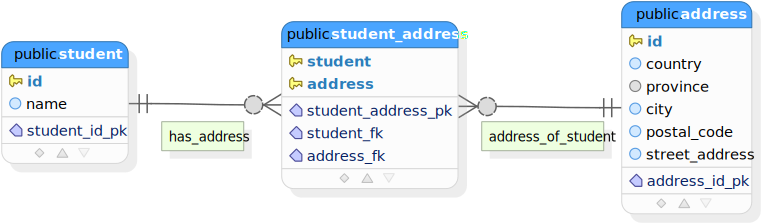
\includegraphics[width=0.85\linewidth]{\currentDir/fixedMultivalued}%
\caption{A redesign of the logical schema from \cref{fig:anomalyMultivalued}. %
Refactoring the multivalued attribute that was represented as repeating group into a separate table brings the model into the \pgls{1NF}.}%
\label{fig:fixedMultivalued}%
\end{figure}%
%
\gitExec{}{\databasesCodeRepo}{.}{_scripts_/postgres.sh normalization/1nf/fixed_multivalued/generated_sql 01_fixed_database_2001.sql}%
\gitExec{}{\databasesCodeRepo}{.}{_scripts_/postgres.sh normalization/1nf/fixed_multivalued/generated_sql 03_public_address_table_5071.sql fixed}%
%
\gitSQL{\databasesCodeRepo}{normalization/1nf/fixed_multivalued/generated_sql/04_public_student_table_5079.sql}{1nf:fixed_multivalued:04_public_student_table_5079}{The generated \sql\ code for creating the \sqlil{student} table, which now only has a primary key and the student name stored.}%
\gitExec{}{\databasesCodeRepo}{.}{_scripts_/postgres.sh normalization/1nf/fixed_multivalued/generated_sql 04_public_student_table_5079.sql fixed}%
%
\gitSQL{\databasesCodeRepo}{normalization/1nf/fixed_multivalued/generated_sql/05_public_student_address_table_5083.sql}{1nf:fixed_multivalued:05_public_student_address_table_5083}{The generated \sql\ code for creating the \sqlil{student_address} table, which has a composite primary key composed of the \sqlil{student} and \sqlil{address} foreign keys. %
The corresponding \sqlilIdx{REFERENCES} constraints have been omitted here for the sake of brevity.}%
%
\gitExec{}{\databasesCodeRepo}{.}{_scripts_/postgres.sh normalization/1nf/fixed_multivalued/generated_sql 05_public_student_address_table_5083.sql fixed}%
%
\gitExec{}{\databasesCodeRepo}{.}{_scripts_/postgres.sh normalization/1nf/fixed_multivalued/generated_sql 06_public_student_address_student_fk_constraint_5087.sql fixed}%
\gitExec{}{\databasesCodeRepo}{.}{_scripts_/postgres.sh normalization/1nf/fixed_multivalued/generated_sql 07_public_student_address_address_fk_constraint_5088.sql fixed}%
%
\gitSQL{\databasesCodeRepo}{normalization/1nf/fixed_multivalued/insert.sql}{1nf:fixed_multivalued:insert}{%
Inserting some data into the tables~\sqlil{student}, \sqlil{address}, and~\sqlil{student_address}.}%
\gitExec{}{\databasesCodeRepo}{.}{_scripts_/postgres.sh normalization/1nf/fixed_multivalued insert.sql fixed}%
%
\gitSQLAndOutput{\databasesCodeRepo}{normalization/1nf/fixed_multivalued}{select.sql}{fixed}{}{}{postgres.sh}{1nf:fixed_multivalued:select}{%
Finding all the students with addresses in China is now easier, as no \sqlilIdx{UNION} is required anymore.}%
%
\gitExec{}{\databasesCodeRepo}{.}{_scripts_/postgres.sh normalization/1nf/fixed_multivalued cleanup.sql}%

So let us fix this problem by extracting the multivalued attribute into a separate table.
For the sake of simplicity, we will not enforce that each student must have at least one address.
We instead create an \crowsFoot{\sqlil{student}}{OM}{\sqlil{address}}{OM} pattern, as discussed back in \dref{sec:rm:op}.
As illustrated in \cref{fig:fixedMultivalued}, we now need a third table, which we will call~\sqlil{student_address}.
This table will have a composite primary key consisting of one foreign key reference to the table~\sqlil{student} and one foreign key reference to the table~\sqlil{address}.
The table~\sqlil{student} is now reduced and its \sqlil{address} attributes are removed.
It now only has its primary key~\sqlil{id} and the student~\sqlil{name} attribute left.
The table~\sqlil{address} stays as it is.

In \cref{lst:1nf:fixed_multivalued:insert}, we first create the \sqlil{address} records.
Then we create the \sqlil{student} records.
Then we insert the relationships between the \sqlil{student} and the \sqlil{address} records in table~\sqlil{student_address}.

Trying to find the students who have at least one address in China now becomes much easier.
The corresponding query, shown in \cref{lst:1nf:fixed_multivalued:select}, does no longer require an \sqlilIdx{UNION} statement.
Instead, we already have the student-address relationships in perfect tabular form.
With only two \sqlilIdx{INNER JOIN} constructs we can make the right connection.
The \sqlilIdx{ILIKE}, \sqlilIdx{ANY}, \sqlilIdx{ARRAY}, and \sqlilIdx{DISTINCT ON} statements are used in the same way as before.

By bringing the data into the \pgls{1NF} we have achieved two things:
First, we made queries significantly simpler.
Second, we also do no longer need to care about the actual number of addresses a student can have.
A student can have one, two, three, four, ten addresses if they want to.
Our query will work all the same.
Of course, a \db\ will not just have one such query.
Maybe there will be another query for students who live in our beautiful city Hefei~(合肥), or for students who do not have any address outside of our Anhui~(安徽) province.
If a student with three addresses had appeared under our old logical schema, then we would need to change the table~\sqlil{student} and then work our way through all of these queries to modify them.
That would have been quite annoying.

That being say, we also have to admit one thing:
I did cheat on you a little bit.
The original schema, which violated the \pgls{1NF}, required each student to have \emph{at least one} address.
The new schema which does not violate the \pgls{1NF} does not.
I said \emph{\inQuotes{For the sake of simplicity, we will now not enforce that each student must have an address.}}
Well, that's a little bit of cheating.
What we \emph{actually} should have implemented is the pattern \crowsFoot{\sqlil{student}}{OM}{\sqlil{address}}{MM}.

When it comes to selecting and querying the data, this changes nothing.
All the advantages mentioned above remain true.
We gain the ability to deal with arbitrary numbers of addresses per student.

However, \emph{inserting} data becomes more complex in a \crowsFoot{Q}{OM}{R}{MM} relationship as compared to a \crowsFoot{O}{OM}{P}{OM} relationship.
We would have needed to use a \sqlilIdx{WITH} statement to simultaneously creating a row in the \sqlil{student} table \emph{and} use the primary key of that row to link this new student record to a row in the table~\sqlil{address}.
It still can be done.
We have learned how to do that.
But if we really want to enforce that each student must have at least one address, then the simple \sqlilIdx{NOT NULL} constraint of the column~\sqlil{address_1} in our original schema must be re-created.
And it is recreated by another foreign key in the table~\sqlil{student}.
For details, please refer back to \cref{sec:rm:qr}.

The interesting aspect of this situation is this:
Usually, normalization makes inserting and updating data easier at the cost of query complexity.
For example, we normalized the composite address attribute into multiple tables.
One annoying aspect here was that we found multiple different spellings of the country \emph{China}.
If we wanted, it would be very very easy to change all the countries to \emph{China} that are either \emph{PRC}, \emph{P.R.C.}, or \emph{中国} with an \sqlilIdx{UPDATE}~statement.
We could do that because we now have the column~\sqlil{country}.
If you want to do that unnormalized \sqlil{address} column than, well, good luck.
We paid for this ease when we want to reassemble the address string, because now we needed to do string concatenation via~\sqlil{||}\sqlIdx{\textbar\textbar} and \sqlilIdx{COALESCE} to deal with \sqlilIdx{NULL}~values.

This time, it is the other way around.
If we had implemented all constraints of the original model, then our \sqlilIdx{INSERT} statements would have become more complicated.
The queries later become much easier.
Either way, our data is certainly \inQuotes{cleaner} and easier to handle in the \pgls{1NF}.%
\FloatBarrier%
\endhsection%
\endhsection%
%
